\section{Auswertung und Diskussion}
\label{sec:AuswertungDiskussion}

\subsection*{Bestrahlungsplan für das PTV1}

Mit dem ersten Bestrahlungsplan wird das PTV1 bestrahlt. Die resultierende Dosisverteilung
ist in den Abbildungen \ref{abb:Z1}, \ref{abb:Y1} und \ref{abb:X1} dargestellt.
Dabei ist die Dosisverteilung aus der transversalen, frontalen und sagittalen Ansicht gezeigt.
Anhand der Dosisverteilung ist zu erkennen, dass obwohl das PTV1 relativ groß ist, es gut gelungen ist das
PTV1 mit der $95\%$ Isodosenlinie zu umschließen. Das PTV1 geht bis zum Anus und da dieser Bereich nah an der Körperoberfläche
liegt, war es in diesem Bereich nicht möglich eine relative Dosis von $95\%$ zu erreichen.
Außerdem ist zu erkennen, dass die maximale relative Dosis $107,6\%$ innerhalb des PTV1 liegt und auch nur minimal
über der erlaubten maximalen Dosis von $107\%$ liegt \cite{ICRU}. Es wird zum Teil auch ausserhalb des PTVs eine hohe relative Dosis deponiert.
Das kommt daher, da das PTV teilweise von Knochen umgeben ist und es somit unvermeidlich ist, dass dort eine hohe Dosis deponiert wird.
Die minimale relative Dosis, die im PTV1 deponiert wird ist $78,9\%$. Diese liegt unterhalb der gewünschten relativen Dosis von $95\%$ und das
liegt zum einen an den bereits beschriebenen Gründen und zum anderen daran, dass die Blase so gut wie möglich geschont werden muss.

\begin{figure}[H]
  \centering
  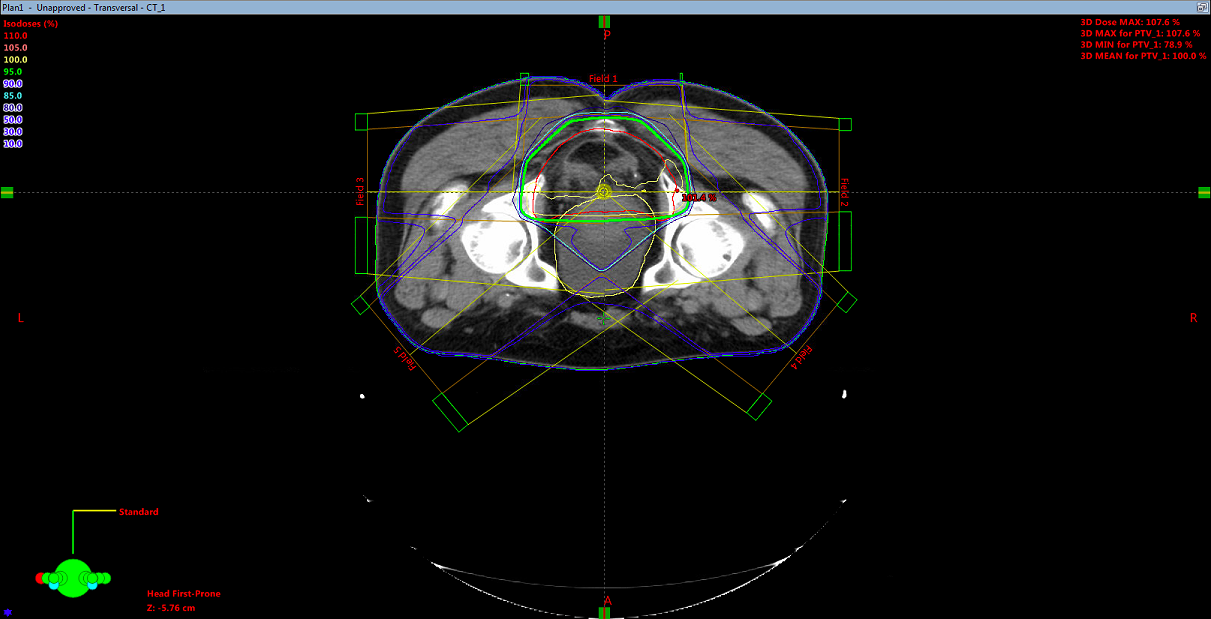
\includegraphics[width=\textwidth]{Bilder/Rektum1_Z.png}
  \caption{Darstellung der Dosisverteilung im Rumpf in Transversalansicht.}
  \label{abb:Z1}
\end{figure}

\begin{figure}[H]
  \centering
  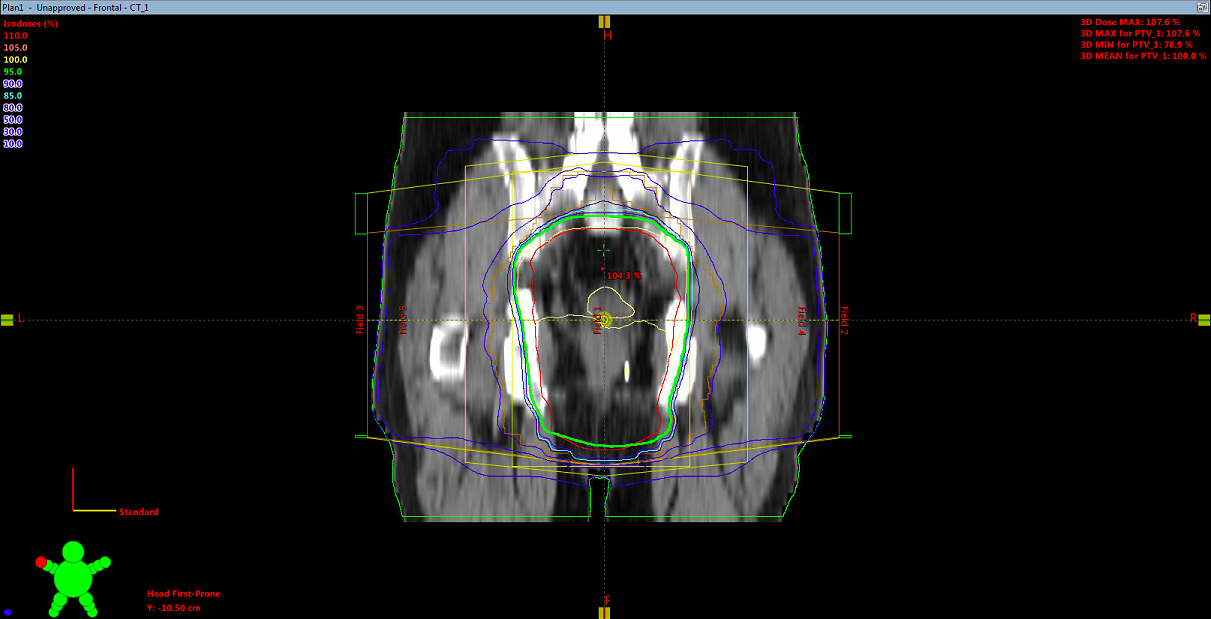
\includegraphics[width=\textwidth]{Bilder/Rektum1_Y.png}
  \caption{Darstellung der Dosisverteilung im Rumpf in Frontalansicht.}
  \label{abb:Y1}
\end{figure}

\begin{figure}[H]
  \centering
  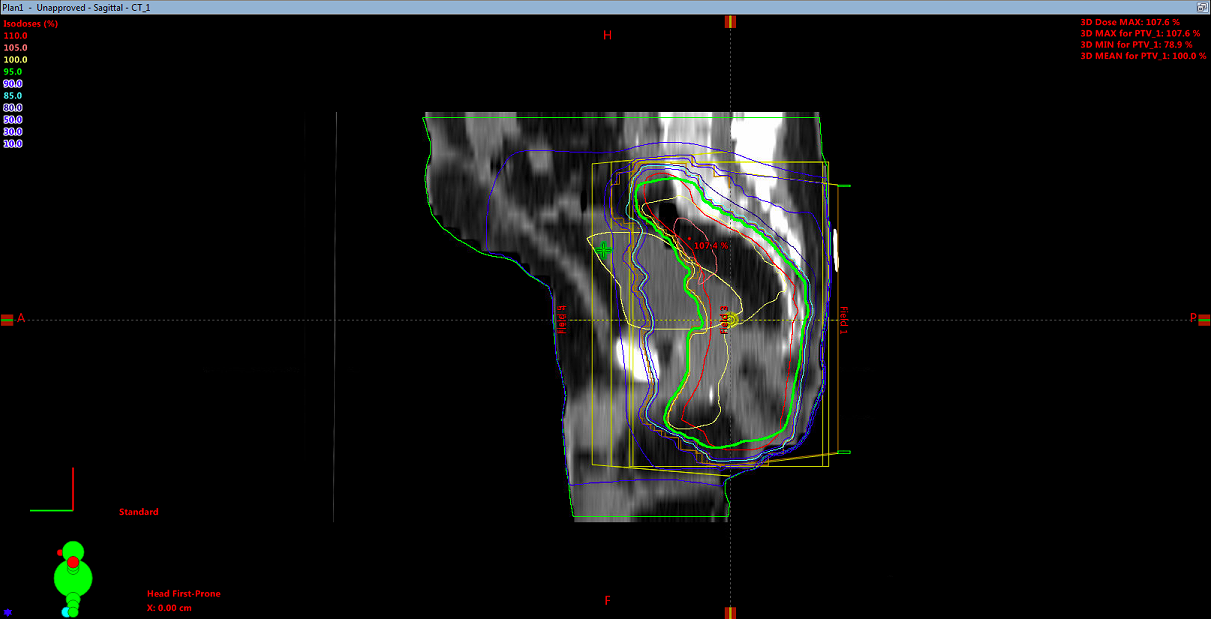
\includegraphics[width=\textwidth]{Bilder/Rektum1_X.png}
  \caption{Darstellung der Dosisverteilung im Rumpf in Sagittalansicht.}
  \label{abb:X1}
\end{figure}

Damit die Dosisverteilung besser beurteilt werden kann, ist in der Abbildung \ref{abb:DVH1} das zugehörige DVH
dargestellt. Anhand der DVH Kurve für das PTV1 (rot) ist zu erkennen, dass nur ein geringer Teil des PTVs eine Dosis von weniger als
$95\%$ erhält. Dadurch, dass die Kurve sehr schnell abfällt wird auch deutlich, dass auch nur ein sehr geringer Teil des PTVs die maximale Dosis erhält.
Bei diesem Bestrahlungsplan ist es nicht gelungen die Blase gut zu schützen. Das ist anhand der gelben DVH Kurve zu erkennen. Die relative maximale Dosis
der Blase liegt bei $105,5\%$ und die DVH Kurve fällt auch nur langsam ab. Auch die Hüftköpfe erhalten eine hohe maximale Dosis von $103,2\%$ und $103,1\%$.
Um zu überprüfen zu können ob die Organdosisgrenzwerte eingehalten worden sind, müssen beide Bestrahlungspläne betrachtet werden. Aus diesem
Grund wird die Dosisverteilung der Risikoorgane am Ende des Protokolls genauer untersucht.
Anhand der DVH Kurve für den gesamten Rumpf (grün) ist zu erkennen, dass das in dem gesamten Gebiet viel Dosis deponiert wird. In etwa $35\%$ des
Rumpfes wird noch eine relative Dosis von $50\%$ deponiert. Das lässt sich nicht vermeiden, da das PTV1 sehr groß ist.

\begin{figure}[H]
  \centering
  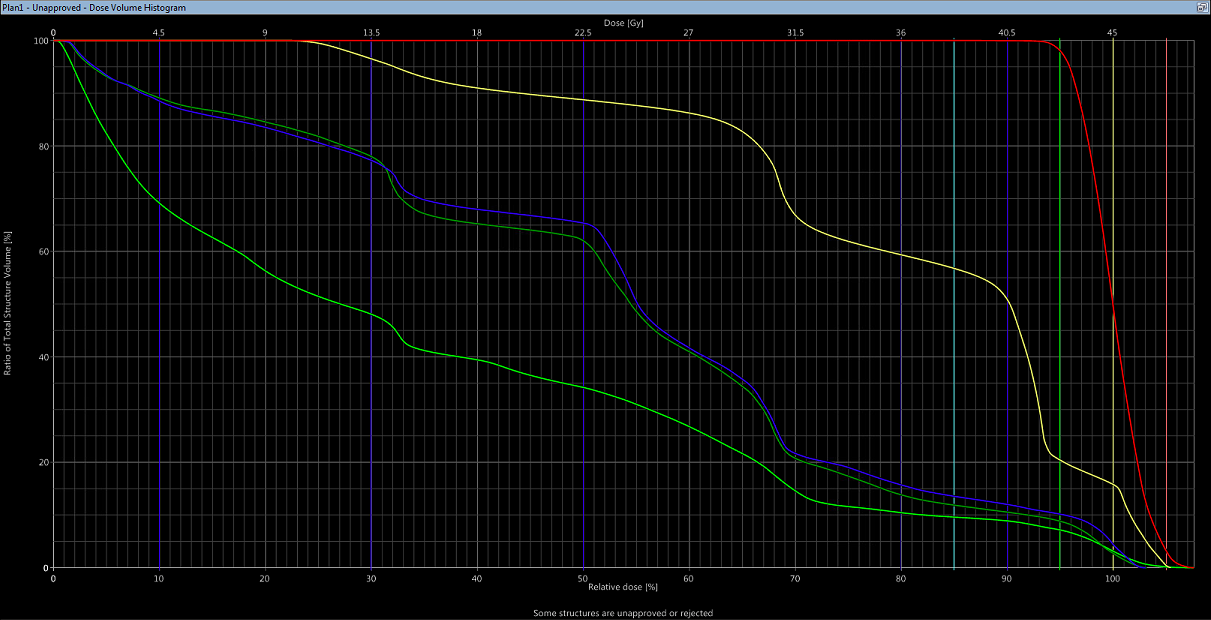
\includegraphics[width=\textwidth]{Bilder/Rektum1_DVH.png}
  \caption{Dosis-Volumen-Histogramm für das PTV1 in rot und den gesamten Rumpf in grün. Außerdem ist das DVH für die Blase in gelb, für den linken Hüftkopf in dunklgrün und für den rechten Hüftkopf in blau dargestellt.}
  \label{abb:DVH1}
\end{figure}

\subsection*{Bestrahlungsplan für das PTV2}

Bei dem zweiten Bestrahlungsplan wird das kleinere PTV2 bestrahlt. Bei dieser zweiten Serie ist die
applizierte Gesamtdosis auch deutlich geringer als bei der ersten Serie.
Die resultierende Dosisverteilung ist in den Abbildungen \ref{abb:Z2}, \ref{abb:Y2} und \ref{abb:X2} gezeigt.
Dabei sind die gleichen Ansichten gezeigt, wie bei dem ersten Plan. Anhand der gezeigten Ansichten der
Dosisverteilung ist zu erkennen, dass das PTV2 gut mit der $95\%$ Isodosenlinie umschlossen werden konnte.
Auch bei diesem Plan liegt die maximale relative Dosis $104,3\%$ innerhalb des PTV2. Diese maximale Dosis liegt unterhalb
der erlaubten maximalen Dosis von $107\%$. Die minimale Dosis in dem PTV2 liegt bei $93\%$. Diese Dosis liegt minimal unterhalb des gewünschten
Dosis von $95\%$.

\begin{figure}[H]
  \centering
  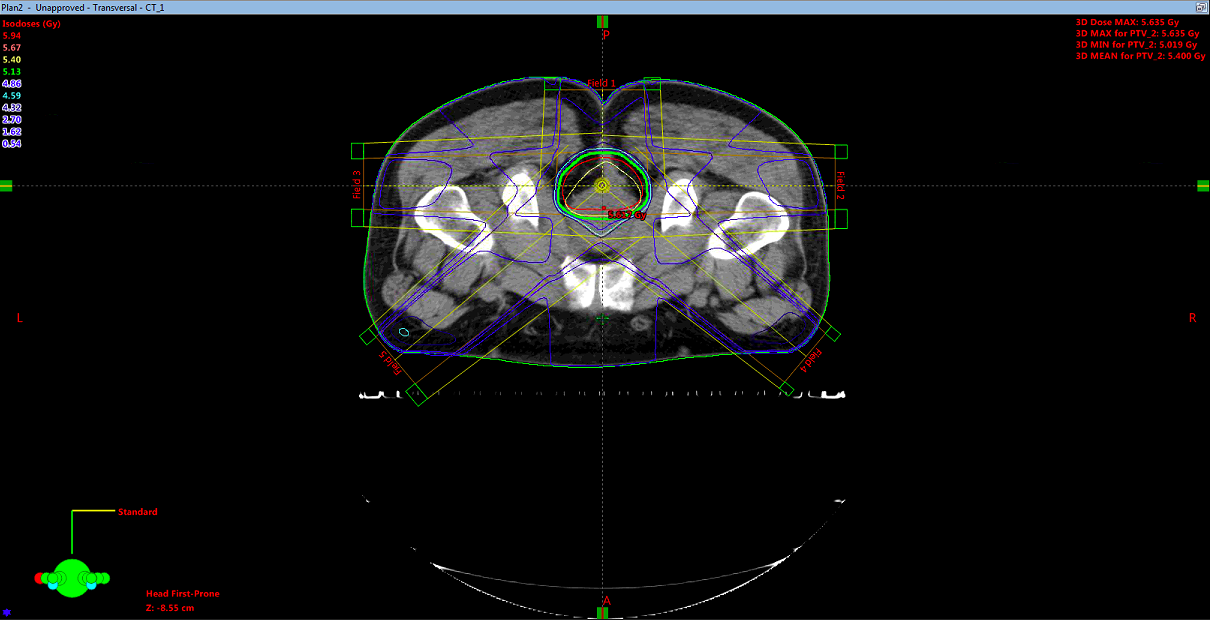
\includegraphics[width=\textwidth]{Bilder/Rektum2_Z.png}
  \caption{Darstellung der Dosisverteilung im Rumpf in Transversalansicht.}
  \label{abb:Z2}
\end{figure}

\begin{figure}[H]
  \centering
  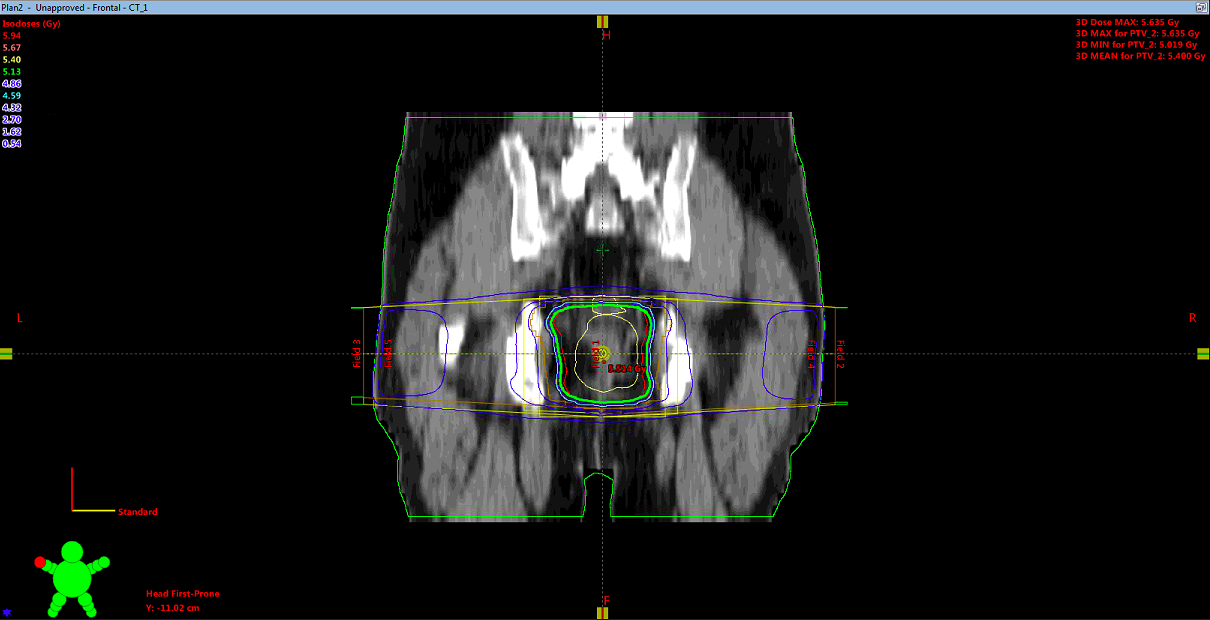
\includegraphics[width=\textwidth]{Bilder/Rektum2_Y.png}
  \caption{Darstellung der Dosisverteilung im Rumpf in Frontalansicht.}
  \label{abb:Y2}
\end{figure}

\begin{figure}[H]
  \centering
  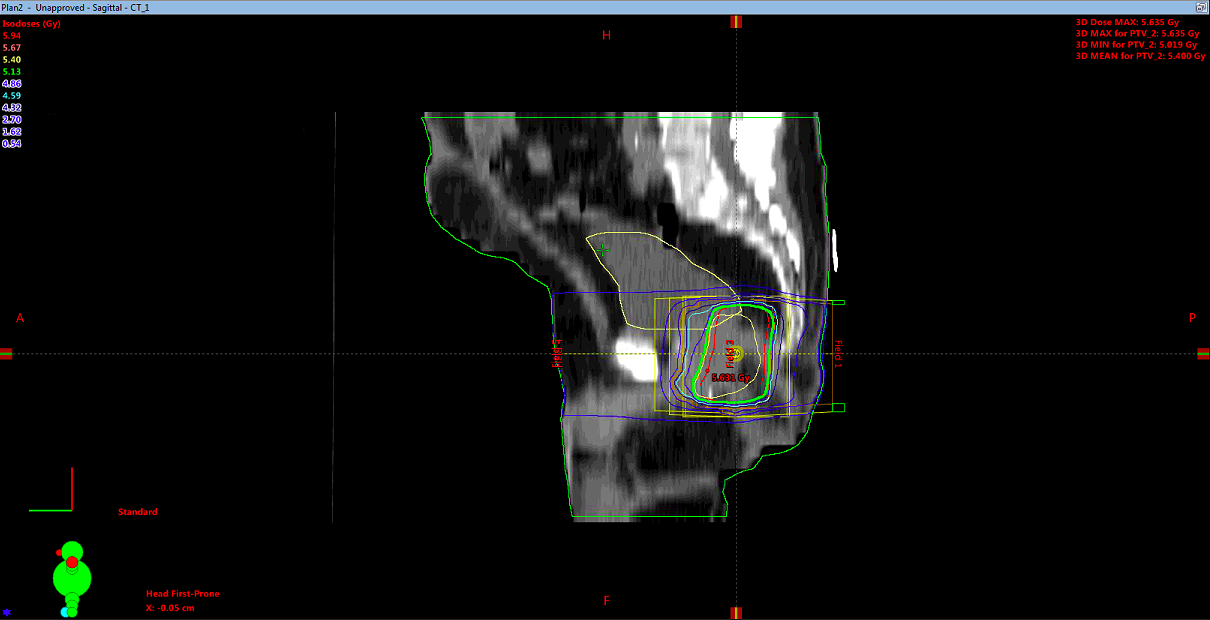
\includegraphics[width=\textwidth]{Bilder/Rektum2_X.png}
  \caption{Darstellung der Dosisverteilung im Rumpf in Sagittalansicht.}
  \label{abb:X2}
\end{figure}

Das zugehörige DVH ist in der Abbildung \ref{abb:DVH2} gezeigt. Anhand des DVHs für das PTV2 (rot)
ist zu erkennen, dass nur ein sehr kleiner Teil des PTVs eine geringere Dosis als $95\%$ erhält.
Außerdem ist anhand des DVHs von dem gesamten Rumpf zu erkennen, dass der Großteil des Rumpfes
nur eine geringe Dosis erhält. Etwa $6\%$ des Rumpfes erhält noch eine relative Dosis von $50\%$.
Anhand der DVH Kurven der Risikoorgane ist zu erkennen, dass diese bei diesem Plan besser geschont werden konnten.
Allerdings ist die relative maximale Dosis der Blase auch hier $101,9\%$ und der Hüftköpfe bei $78,3\%$ und $96,9\%$.
Im folgenden wird die Summe der beiden Pläne betrachtet um beurteilen zu können ob die Organdosisgrenzwerte eingehalten
worden sind.

\begin{figure}[H]
  \centering
  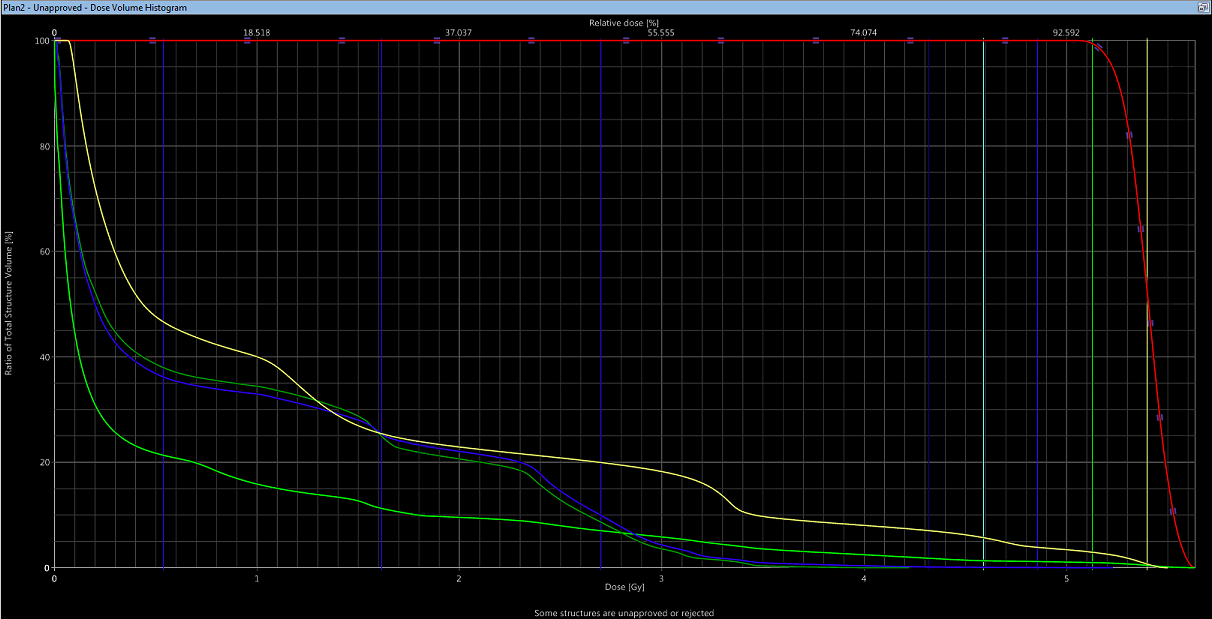
\includegraphics[width=\textwidth]{Bilder/Rektum2_DVH.png}
  \caption{Dosis-Volumen-Histogramm für das PTV2 in rot und den gesamten Rumpf in grün. Außerdem ist das DVH für die Blase in gelb, für den linken Hüftkopf in dunklgrün und für den rechten Hüftkopf in blau dargestellt.}
  \label{abb:DVH2}
\end{figure}

\subsubsection*{Summe der Bestrahlungspläne}

In der Abbildung \ref{abb:DVHsum} ist das DVH der Summe der beiden Bestrahlungspläne dargestellt.
Die Organdosisgrenzwerte werden aus der QUANTEC Tabelle entnommen \cite{QUANTEC}. Der Grenzwert für die
Blase beträgt $\SI{65}{\gray}$ und bei den Hüftköpfen darf nur weniger als $10\%$ des Volumens eine Dosis von $\SI{52}{\gray}$ erhalten.
Anhand des DVHs der Summe
der beiden Bestrahlungspläne ist zu erkennen, dass die Blase insgesamt eine maximale Dosis von
$\SI{50.989}{\gray}$ erhält. Diese Dosis liegt noch deutlich unterhalb des Grenzwertes.
Die Hüftköpfe erhalten eine maximale Dosis von $\SI{49.695}{\gray}$ und $\SI{50.349}{\gray}$.
Auch diese Dosen liegen unterhalb des Grenzwertes.

\begin{figure}[H]
  \centering
  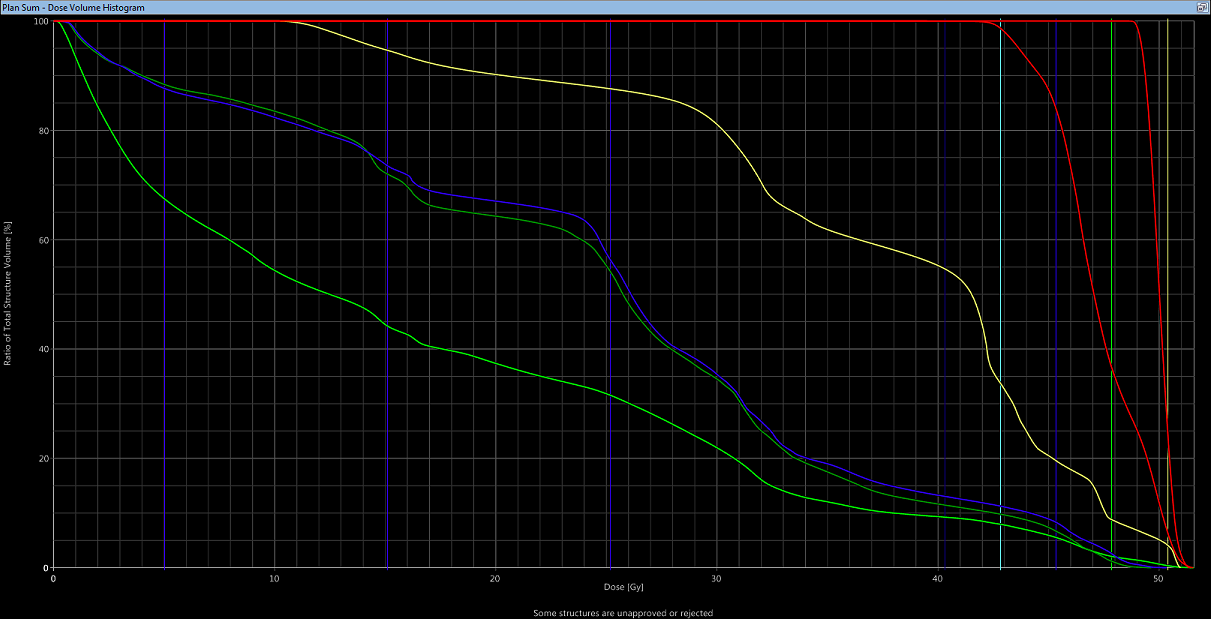
\includegraphics[width=\textwidth]{Bilder/Rektum_summe.png}
  \caption{Dosis-Volumen-Histogramm für die Summe der beiden Bestrahlungspläne. Für das PTV1 und PTV2 in rot und den gesamten Rumpf in grün. Außerdem ist das DVH für die Blase in gelb, für den linken Hüftkopf in dunkelgrün und für den rechten Hüftkopf in blau.}
  \label{abb:DVHsum}
\end{figure}

Insgesamt wurden bei dieser Bestrahlungsplanung relativ viele Felder verwendet um eine
akzeptable Dosisverteilung zu erreichen. Durch die Verwendung von MLCs ist es gelungen
die Organdosisgrenzwerte der Blase und der Hüftköpfe nicht zu überschreiten.
Außerdem ist das PTV in beiden Bestrahlungsplänen hinreichend mit der $95\%$ Isodosenlinie
umschlossen worden.
